\newpage
\subsection{Recall}
    Following are the recall @ i curves. Plots are shown for both ACMR\cite{acmr} and OCMFH\cite{ocmfh} on various datasets(nuswide, xmedianet, and wiki) with varying bit vector length.
        \begin{figure}[H]
            \begin{minipage}[!h]{0.5\linewidth}
                \centering
                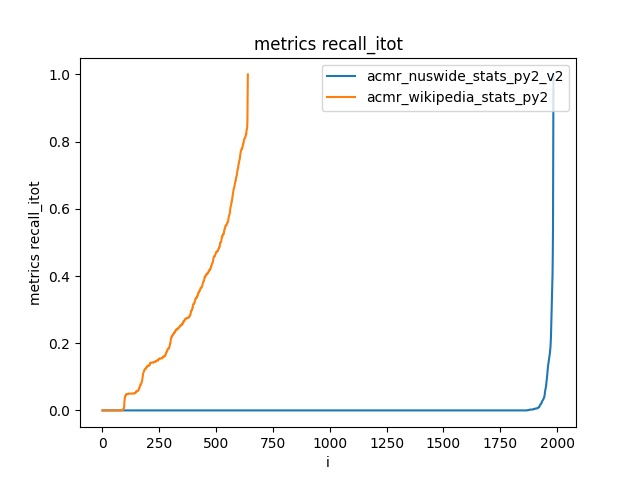
\includegraphics[width=\linewidth]{resultsImages/recall/metrics recall_itot_acmr_both.jpeg}
                % \caption{Query type: min}
                % \label{fig:six_core_min}
                % \vspace{0.1ex}
                % \hspace{0ex}
            \end{minipage}
            \begin{minipage}[!h]{0.5\linewidth}
                \centering
                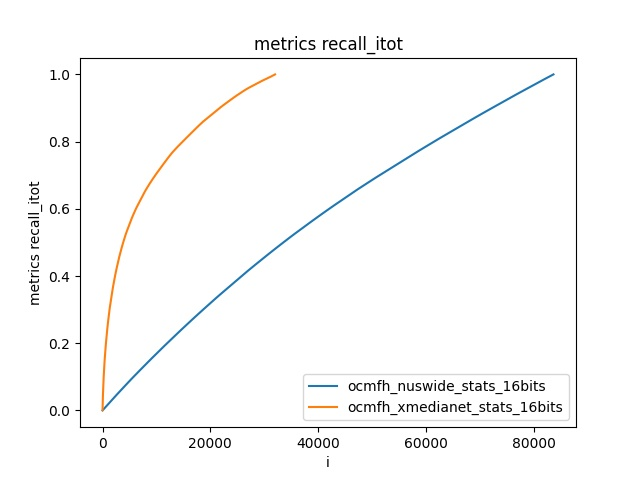
\includegraphics[width=\linewidth]{resultsImages/recall/metrics recall_itot_ocmfh_both.jpeg}
                % \caption{Query type: sum}
                % \label{fig:six_core_sum}
                % \vspace{0.1ex}
                % \hspace{0ex}
            \end{minipage}
            \begin{minipage}[!h]{0.5\linewidth}
                \centering
                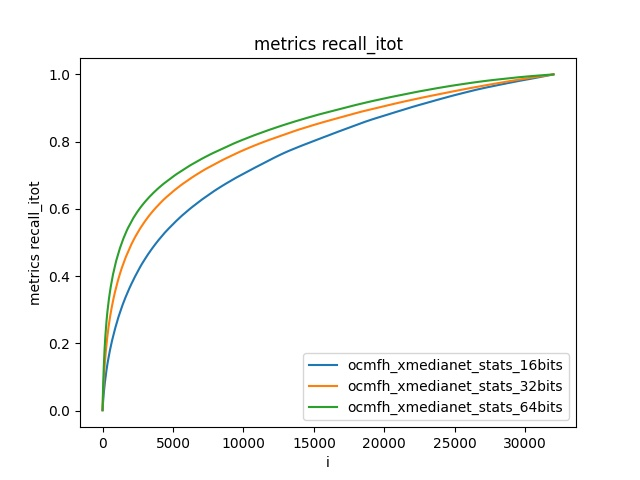
\includegraphics[width=\linewidth]{resultsImages/recall/metrics recall_itot_ocmfh_xmedia.jpeg}
                % \caption{Query type: countrange}
                % \label{fig:six_core_countrange}
                % \vspace{0.1ex}
                % \hspace{0.1ex}
            \end{minipage}
            \begin{minipage}[!h]{0.5\linewidth}
                \centering
                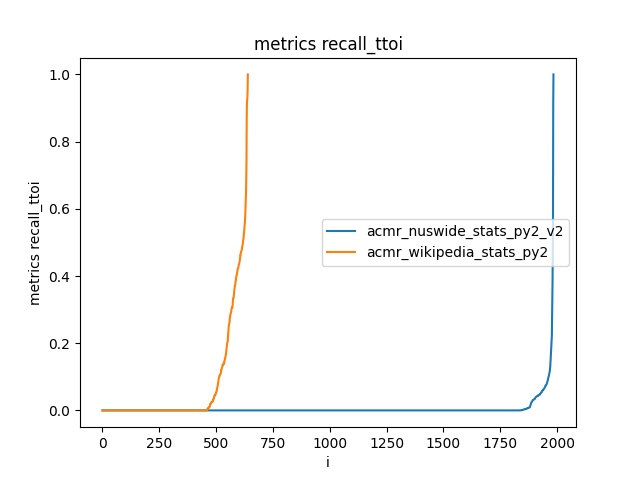
\includegraphics[width=\linewidth]{resultsImages/recall/metrics recall_ttoi_acmr_both.jpeg}
                % \caption{Query type: max}
                % \label{fig:six_core_max}
                % \vspace{0.1ex}
                % \hspace{0.1ex}
            \end{minipage}
            
            \begin{minipage}[!h]{0.5\linewidth}
                \centering
                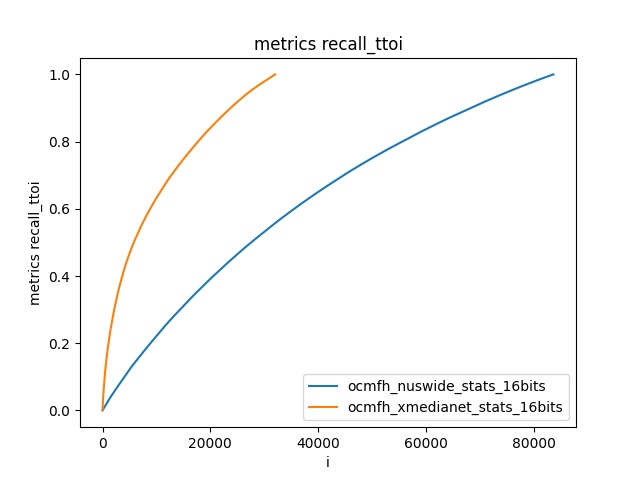
\includegraphics[width=\linewidth]{resultsImages/recall/metrics recall_ttoi_ocmfh_both.jpeg}
                % \caption{Query type: countrange}
                % \label{fig:six_core_countrange}
                % \vspace{0.1ex}
                % \hspace{0.1ex}
            \end{minipage}
            \begin{minipage}[!h]{0.5\linewidth}
                \centering
                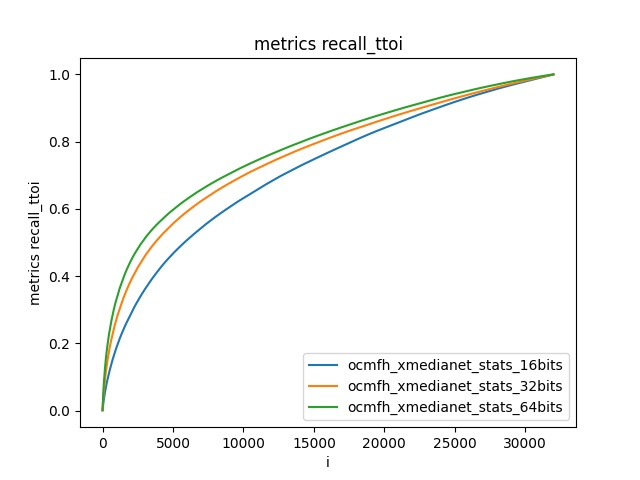
\includegraphics[width=\linewidth]{resultsImages/recall/metrics recall_ttoi_ocmfh_xmedia.jpeg}
                % \caption{Query type: max}
                % \label{fig:six_core_max}
                % \vspace{0.1ex}
                % \hspace{0.1ex}
            \end{minipage}
        \caption{Recall metric for ACMR and OCMFH on various datasets}
        \label{fig:}
        \end{figure}
        \FloatBarrier